\chapter{Casi d'uso}

\section{UC1}

\section{UC2 - Selezione tipo di grafico}
\begin{figure}[H]
 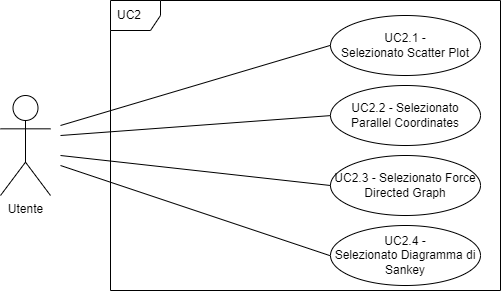
\includegraphics[width=\textwidth]{uc2.png}
 \vspace{-5mm}
 \caption*{Figura 2: UC2 - Selezione tipo di grafico}
\end{figure}
 \begin{itemize}
     \item \textbf{Attore primario:} Utente.
     \item \textbf{Precondizioni:} Il sistema è stato inizializzato [UC1].
     \item \textbf{Postcondizioni:} Scelta delle dimensioni del grafico [UC3].
     \item \textbf{Scenario principale:} L'utente sceglie la visualizzazione più consona tra quelle disponibili.
     \item \textbf{Generalizzazioni:} L'utente può selezionare una delle seguenti opzioni:
     \begin{enumerate}
         \item \textit{Scatter Plot} [UC2.1]
         \item \textit{Parallel Coordinates} [UC2.2]
         \item \textit{Force Directed Graph} [UC2.3]
         \item \textit{Diagramma di Sankey} [UC2.4]
     \end{enumerate}
 \end{itemize}
 
 \subsection{UC2.1 - Selezionato Scatter Plot}
  \begin{itemize}
      \item \textbf{Attore Primario:} Utente.
      \item \textbf{Precondizioni:} Il sistema è stato inizializzato [UC1].
      \item \textbf{Postcondizioni:} Viene mostrata la scelta delle dimensioni del grafico [UC3].
      \item \textbf{Scenario principale:} L'utente seleziona la visualizzazione \textit{Scatter Plot} e il sistema ritorna la selezione della dimensione.
  \end{itemize}
 \subsection{UC2.2 - Selezionato Parallel Coordinates}
 \begin{itemize}
    \item \textbf{Attore Primario:} Utente.
    \item \textbf{Precondizioni:} Il sistema è stato inizializzato [UC1].
    \item \textbf{Postcondizioni:} Viene mostrata la scelta delle dimensioni del grafico [UC3].
    \item \textbf{Scenario principale:} L'utente seleziona la visualizzazione \textit{Parallel Coordinates} e il sistema ritorna la selezione della dimensione.
\end{itemize}
 \subsection{UC2.3 - Force Directed Graph}
 \begin{itemize}
    \item \textbf{Attore Primario:} Utente.
    \item \textbf{Precondizioni:} Il sistema è stato inizializzato [UC1].
    \item \textbf{Postcondizioni:} Viene mostrata la scelta delle dimensioni del grafico [UC3].
    \item \textbf{Scenario principale:} L'utente seleziona la visualizzazione \textit{Force Directed Graph} e il sistema ritorna la selezione della dimensione.
\end{itemize}
 \subsection{UC2.4 - Diagramma di Sankey}
 \begin{itemize}
    \item \textbf{Attore Primario:} Utente.
    \item \textbf{Precondizioni:} Il sistema è stato inizializzato [UC1].
    \item \textbf{Postcondizioni:} Viene mostrata la scelta delle dimensioni del grafico [UC3].
    \item \textbf{Scenario principale:} L'utente seleziona la visualizzazione \textit{Diagramma di Sankey} e il sistema ritorna la selezione della dimensione.
\end{itemize}

\section{UC3}

\section{UC4}

\section{UC5}

\section{UC6}

\section{UC7}